\chapter[Proposta]{Proposta}
\label{ch:proposta}
\section{Considerações Iniciais }

A ideia sobre o domínio ciclo menstrual e atividades surgiu a 
partir de um video\footnote{video :https://www.youtube.com/watch?v=sNRi9A6LaHM. Último acesso em: 03/12/2020} em que a palestrante comenta sobre um 
trabalho que ela estava desenvolvendo com mais duas  
mulheres e que elas gerenciaram o projeto, delegando tarefas, de 
acordo com o ciclo menstrual de cada uma. Levantam a hipótese de 
que em cada fase do ciclo menstrual, cada mulher tem um tipo 
de comportamento e por isso, nessas fases, algumas atividades 
podem ser mais produtivas.
A própria autora deste trabalho começou a notar então, na sua 
vivência, que certos padrões se repetiam, ciclo após ciclo.

Essa inspiração foi levada aos 
orientadores, e começaram a ser discutidas possíveis aplicações da 
engenharia de software sobre o domínio. Duas ideias centrais 
foram levantadas. 

A primeira ideia foi utilizar aprendizado de máquina para 
acordar um perfil comportamental com base no ciclo menstrual e 
com isso conferir previsões sobre produtividade, humor, sintomas 
físicos e entre outros. Essa ideia foi descartada porque para 
um bom desempenho de um aprendizado de máquina, seria necessário 
uma base de dados volumosa, dados esses que 
a autora não continha. Além disso, o termo produtividade também 
foi descartado por envolver uma medida muito subjetiva e questões éticas e morais. 

A segunda ideia surgiu baseada no trabalho de \citeonline{leticia}, Sistema de Recomendação para Atribuição de Tarefas de Testes 
Baseado em Perfil de Testadores, que levantou a questão se seria 
possível desenvolver um tema similar, só que no
contexto de recomendações de tarefas baseadas no perfil e 
ciclo menstrual. A segunda ideia foi a escolhida para ser 
utilizada para o desenvolvimento deste trabalho.

Algumas problemáticas sobre o tema foram levantadas. A primeira 
foi, o trabalho vai contar com o acompanhamento de um 
profissional da área da saúde? Optou-se por não envolver 
terceiros no desenvolvimento do trabalho, por causa da 
burocracia envolvida e da dificuldade 
em encontrar uma pessoa com disponibilidade e interesse em 
acompanhar o projeto. A segunda problemática foi, 
como adquirir os dados necessários para desenvolver um 
Sistema de Recomendação? Optou-se por criar um grupo 
específico que servirá como estudo de caso, participando tanto 
da coleta de dados quanto dos testes da aplicação. O estudo de 
caso também resolveu, de certa forma, a primeira problemática, 
porque delimitou o desenvolvimento da aplicação para um grupo 
específico de pessoas. 


\section{Coleta de Dados}

Um grupo com 23 mulheres que se interessaram pelo tema foi criado. A primeira 
atividade com o grupo envolveu discussões de como as colaboradoras se sentiam durante as fases. Foi orientado
às participantes que ficassem mais atentas às mudanças e como elas influenciavam na realização de 
atividades cotidianas. Para que elas se sentissem mais confortáveis realizando a tarefa, o método para tomar notas ficou a cargo de cada uma. 
Algumas começaram a anotar em uma agenda e outras utilizaram 
aplicativos de ciclo menstrual já existentes no mercado. Ficou acordado que, 
nesse momento, as notas não precisam ser compartilhadas e que, posteriormente, o grupo seria aberto para 
aquelas que se sentissem confortáveis em compartilhar o que perceberam 
durante esse trabalho interno.

As discussões com o grupo e o estudo inicial da referência bibliográfica foram então utilizados para 
delimitar questões que seriam aplicadas à primeira coleta de dados a partir de um questionário.

\subsection{Definição da Plataforma}

Após expor ao grupo o tema do trabalho, foi realizada uma enquete para definir que tipo de plataforma as 
integrantes preferiam para o desenvolvimento da aplicação. A Figura \ref{fig07} traz o resultado da enquete. Ficou definido, então, que seria 
um aplicativo.

\begin{figure}[h]
	\centering
	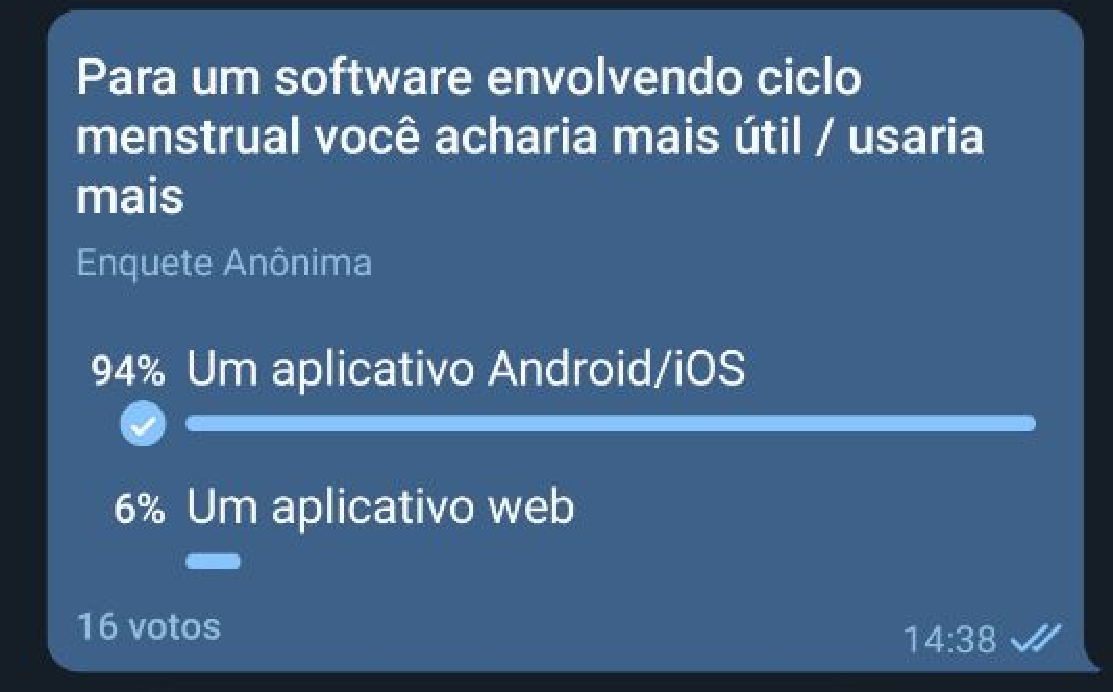
\includegraphics[keepaspectratio=true,scale=0.3]{figuras/enqueteApp.pdf}
	\caption{Enquete Sobre a Aplicação}
        \label{fig07}
\end{figure}

\subsection{Questões do Questionário}

A Tabela \ref{tab06} e a Tabela \ref{tab07} apresentam as questões que foram utilizadas para o primeiro ciclo de coleta de dados sobre o ciclo menstrual e 
sua influência. O questionário\footnote{questionário : https://forms.gle/4Q3HoyXydcY89TjY9} foi feito utilizando a plataforma Google Forms e foi respondido de forma anônima, para que as
participantes se sentissem mais confortáveis respondendo-o. Ao todo, o questionário contou com 31 perguntas, sendo 20 fechadas e 
11 abertas. Foram recebidas 23 respostas até a data 18/03/2020.

\begin{table}[h]
	\centering
	\caption{Perguntas Fechadas do Questionário}
	\label{tab06}
	\begin{tabular}{c}
		\toprule
		\textbf{Perguntas fechadas} \\
        \midrule
        \begin{minipage} [t] {1\textwidth} Qual a sua Idade?  \end{minipage} \\
        \midrule
        \begin{minipage} [t] {1\textwidth} Você utiliza algum método contraceptivo hormonal?   \end{minipage}\\
        \midrule
        \begin{minipage} [t] {1\textwidth} Você utiliza algum método contraceptivo não hormonal?  \end{minipage} \\
        \midrule
        \begin{minipage} [t] {1\textwidth}  Você tem algum distúrbio endócrino como ovários policísticos? Ou outros? \end{minipage}  \\
        \midrule
        \begin{minipage} [t] {1\textwidth}  Você monitora o seu ciclo? \end{minipage}\\
        \midrule
        \begin{minipage} [t] {1\textwidth}  Como você monitora o seu ciclo? \end{minipage} \\
        \midrule
        \begin{minipage} [t] {1\textwidth}  Você iria preferir uma aplicação para monitorar o seu ciclo?\end{minipage}\\
        \midrule
        \begin{minipage} [t] {1\textwidth}  Qual o tamanho do seu ciclo? \end{minipage}\\
        \midrule
        \begin{minipage} [t] {1\textwidth}  Você sente que de alguma forma seu ciclo influencia sua produtividade em certas atividades do dia-a-dia? \end{minipage}\\
        \midrule
        \begin{minipage} [t] {1\textwidth}  Em uma escala de 0 a 4 o quanto você acha que o seu ciclo influência na produtividade do dia-a-dia? \end{minipage}\\
        \midrule
        \begin{minipage} [t] {1\textwidth} Se sim, como identifica? Há alguma alteração de humor, comportamental ou sintoma físico? Tem alterações de humor dependendo da fase do seu ciclo menstrual? \end{minipage}\\
        \midrule
        \begin{minipage} [t] {1\textwidth} Você costuma ter alterações comportamentais dependendo da fase do seu ciclo Menstrual? \end{minipage}\\
        \midrule
        \begin{minipage} [t] {1\textwidth} Você costuma ter algum sintoma físico dependendo da fase do seu ciclo menstrual? \end{minipage}\\
        \midrule
        \begin{minipage} [t] {1\textwidth} Seu fluxo durante a menstruação é:\end{minipage}\\
        \midrule
        \begin{minipage} [t] {1\textwidth} Você costuma ter alguma alteração de humor, sintoma físico, ou alteração comportamental durante a menstruação? \end{minipage}\\
        \midrule
        \begin{minipage} [t] {1\textwidth} Você costuma ter alguma alteração de humor, sintoma físico, ou alteração comportamental durante a fase folicular? \end{minipage}\\
        \midrule
        \begin{minipage} [t] {1\textwidth} Você consegue identificar sua ovulação? \end{minipage}\\
        \midrule
        \begin{minipage} [t] {1\textwidth} Você costuma enfrentar sintomas da TPM? \end{minipage}\\
        \midrule
        \begin{minipage} [t] {1\textwidth} Por quanto tempo você enfrenta os sintomas da TPM antes da menstruação? \end{minipage}\\
        \midrule
        \begin{minipage} [t] {1\textwidth} Qual a intensidade dos seus sintomas da TPM? \end{minipage}\\
		\bottomrule
	\end{tabular}
\end{table}


\begin{table}[h]
	\centering
	\caption{Perguntas Abertas do Questionário}
    \label{tab07}
	\begin{tabular}{c}
		\toprule
		\textbf{Perguntas abertas} \\
		\midrule     
        \begin{minipage} [t] {1\textwidth}  O que mais utiliza ou mais gosta nas aplicações que utiliza para monitorar o seu ciclo? \end{minipage} \\
        \midrule
        \begin{minipage} [t] {1\textwidth} Quais atividades você normalmente realiza no seu dia-a-dia, frequentemente ou de forma cíclica? \end{minipage}\\
        \midrule
        \begin{minipage} [t] {1\textwidth} Descreva os sintomas que você nota que aparecem durante a menstruação\end{minipage}\\
        \midrule
        \begin{minipage} [t] {1\textwidth} Descreva algumas atividades que ficam mais fáceis ou mais difíceis de serem realizadas durante a menstruação.\end{minipage}\\
        \midrule
        \begin{minipage} [t] {1\textwidth} Descreva os sintomas que você nota que aparecem durante a fase folicular.\end{minipage}\\
        \midrule
        \begin{minipage} [t] {1\textwidth} Descreva algumas atividades que ficam mais fáceis ou mais difíceis de serem realizadas durante a fase folicular.\end{minipage}\\
        \midrule
        \begin{minipage} [t] {1\textwidth} Como identifica a ovulação? Há alguma alteração de humor, comportamental ou sintoma físico? \end{minipage}\\
        \midrule
        \begin{minipage} [t] {1\textwidth} Descreva algumas atividades que ficam mais fáceis ou mais difíceis de serem realizadas durante a ovulação.\end{minipage}\\
        \midrule
        \begin{minipage} [t] {1\textwidth} Descreva os sintomas que você nota que aparecem durante a TPM.\end{minipage}\\
        \midrule
        \begin{minipage} [t] {1\textwidth} Descreva algumas atividades que ficam mais fáceis ou mais difíceis de serem realizadas durante a TPM.\end{minipage}\\
        \midrule
        \begin{minipage} [t] {1\textwidth} Caso deseje compartilhar alguma informação que não foi abordada nas perguntas, mas que considera ser relevante para o tema, compartilhe comigo. \end{minipage}\\

		\bottomrule
	\end{tabular}
\end{table}


\section{Análise de Dados}

A tabulação \footnote{tabulação do questionário:https://docs.google.com/document/d/1P7QGKI53WTkpyMegsE} do questionário foi realizada utilizando o Google Docs para escrita e Google Excel para montagem dos gráficos não oferecidos 
pelo Google Forms. A partir dessa tabulação, foi possível extrair informações dos perfis, sintomas e tarefas que iriam compor o sistema de recomendação.

\subsection{Extração de Informação dos Perfis}

Alguns perfis foram identificados a partir do questionário e são listados na Tabela \ref{tab08}. Algumas dessas perguntas irão compor o questionário inicial do aplicativo, para calibração. Quais 
dessas perguntas serão certamente utilizadas, irão ser definidas no escopo do TCC2. 

Basicamente, quase todos os perfis têm sintomas durante todas as fases, menos quando se trata da ovulação, porque aquelas 
que utilizam métodos contraceptivos hormonais não ovulam. Aquelas que utilizam métodos contraceptivos hormonais e não possuem 
distúrbios endócrinos relataram não ter mudança de humor durante os ciclos.

\begin{table}[]
    \caption{Perfis Mapeados}
    \label{tab08}
    \begin{tabular}{|l|c|c|c|c|}
    \hline
    \rowcolor[HTML]{C0C0C0} 
     Perguntas & Perfil 1 & Perfil 2 & Perfil 3 & Perfil 4 \\ \hline
     Utiliza método contraceptivo hormonal?& sim & sim & nao & nao \\ \hline
    \rowcolor[HTML]{EFEFEF} 
    Possui distúrbio endócrino? & sim & não & sim & nao \\ \hline
    Ciclo regular? & sim & sim & não & sim \\ \hline
    \rowcolor[HTML]{EFEFEF} 
    Alteração de humor? & sim & não & sim & sim \\ \hline
    Alteração comportamental? & sim & sim & sim & sim \\ \hline
    \rowcolor[HTML]{EFEFEF} 
    Sintomas físicos? & sim & sim & sim & sim \\ \hline
    Sintomas de TPM? & sim & sim & sim & sim \\ \hline
    \rowcolor[HTML]{EFEFEF} 
    Alterações na fase lútea? & sim & sim & sim & sim \\ \hline
    Alterações na fase folicular? & sim & sim & sim/não & sim/não \\ \hline
    \rowcolor[HTML]{EFEFEF} 
    Alteração no período menstrual? & sim & sim & sim/não & sim/não \\ \hline
    \end{tabular}
    \end{table}

\subsection{Tarefas a Serem Recomendadas}

Através das perguntas abertas e do estudo do referencial teórico (Capítulo \ref{ch:referencial}), 
foi possível mapear, de forma generalista, quais tarefas seriam 
recomendadas 
como mais fáceis ou mais difíceis, ou seja, precisam de 
mais ou menos energia para serem executadas em determinada fase. 

Na Tabela \ref{tab09} seta $\uparrow$ indica menor gasto de energia
(tarefas mais fáceis); a seta $\downarrow$ indica maior gasto de 
energia(tarefas mais difíceis), e - para neutro.

No escopo do TCC2, será realizado mais um questionário específico para as 
tarefas. Essas tarefas poderão ser, então, mais bem classificadas de acordo 
com os perfis.

\begin{table}[]
    \centering
	\caption{Relação de Tarefas mais Fáceis e mais Dificeis}
    \label{tab09}
    \begin{tabular}{|l|c|c|c|c|}
    \hline
    \rowcolor[HTML]{C0C0C0} 
    \multicolumn{1}{|c|}{\cellcolor[HTML]{C0C0C0}Tarefas recomendadas}  & Menstruação & Fase folicular  & Fase lútea & TPM \\ \hline
    Estudar & $\downarrow$  & $\uparrow$ & $\uparrow$ & $\downarrow$ \\ \hline
    \rowcolor[HTML]{EFEFEF} 
    Trabalhar & $\downarrow$ & $\uparrow$  & $\uparrow$ &  $\downarrow$  \\ \hline
    Exercitar & $\downarrow$ & $\uparrow$ & $\uparrow$ &  $\downarrow$  \\ \hline
    \rowcolor[HTML]{EFEFEF} 
    Arrumar a casa  & $\downarrow$ & $\uparrow$  & - & - \\ \hline
    Ler & $\uparrow$ & -  & - & - \\ \hline
    \rowcolor[HTML]{EFEFEF} 
    Fazer reuniões & - & $\uparrow$ & $\downarrow$ & $\downarrow$ \\ \hline
    \rowcolor[HTML]{EFEFEF} 
    Socializar & $\downarrow$ & $\uparrow$  & $\downarrow$ & $\downarrow$ \\ \hline
    \rowcolor[HTML]{EFEFEF} 
    Escrever & - & $\uparrow$  & - & - \\ \hline
    Ouvir música & - & - & - & $\uparrow$ \\ \hline
    \rowcolor[HTML]{EFEFEF} 
    Assistir séries/Tv & $\uparrow$ & - & - & $\uparrow$ \\ \hline
    Desenhar & $\uparrow$ & $\uparrow$  & - & - \\ \hline
    \rowcolor[HTML]{EFEFEF} 
    Criar & - & $\uparrow$  & - & - \\ \hline
    \end{tabular}
    \end{table}

\section{O Aplicativo}

A usuária, após fazer o cadastro, deverá responder a um pequeno 
questionário para coletas iniciais de dados. Isso ajudará a reduzir 
o problema do começo frio, e fornecer informações importantes 
como data da última menstruação, quanto tempo dura a menstruação 
e se possui sintomas de TPM.

A data da última menstruação é importante para utilizar o 
método do calendário, descrito no referencial teórico (Capítulo \ref{ch:referencial}). 
Esse método é o que será utilizado para determinar em que 
fase do ciclo a usuária se encontra.

\subsection{Prova de Conceito}
 
Como prova de conceito, foi desenvolvido um protótipo de alta 
fidelidade utilizando o Figma. Foi desenvolvida uma primeira versão da tela principal, 
com o objetivo de demonstrar a possível 
realização deste trabalho. Os requisitos foram elicitados 
a partir do questionário, que 
originou um \emph{Rich Picture} para facilitar na apresentação dos mesmos, conforme ilustrado na Figura \ref{fig08}.

\begin{figure}[h]
	\centering
	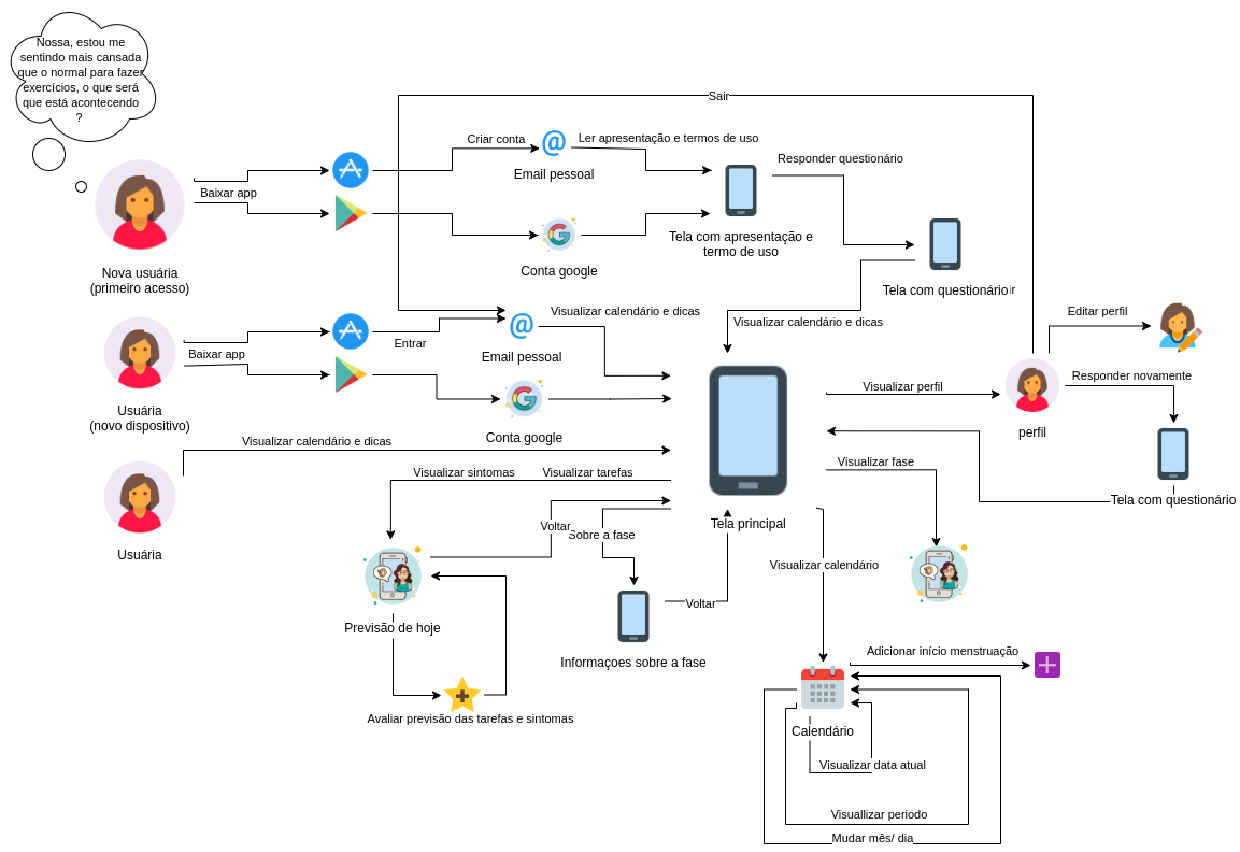
\includegraphics[keepaspectratio=true,scale=0.8]{figuras/rickPicture.pdf}
	\caption{\emph{Rich Picture}}
        \label{fig08}
\end{figure}

\subsection{\emph{Product Backlog}}
Como uma forma de modelagem de acordo com a metodologia Scrum, 
um \emph{product backlog} foi construído utilizando um total de 
sete temas: conta, questionário, sobre a fase, previsão, perfil, 
calendário e documentação. Um maior 
detalhamento, com histórias de usuário, será realizado no 
escopo do TCC2.

\begin{itemize}
    \item P01: Conta -> envolverá a parte de criar uma conta nova e entrar em uma conta já existente;
    \item P02: Questionário -> envolverá a criação do questionário inicial do aplicativo e sua possível edição;
\item P03: Sobre a Fase -> envolverá a criação de textos informativos sobre a fase;
\item P04: Previsão -> envolverá a sugestão de tarefas e sintomas que podem aparecer na respectiva fase do ciclo;
\item P05: Perfil -> envolverá a edição do perfil, como mudança de senha e configurações;
\item P06: Calendário -> envolverá a criação do calendário que mostrará o ciclo completo e as fases, e
\item P07: Documentação -> envolverá toda a atividade de documentação do aplicativo.

\end{itemize}


\subsubsection{Protótipo de Alta Fidelidade}

O protótipo de alta fidelidade conta com a apresentação 
inicial do aplicativo com a logo. Depois, a usuária 
pode escolher entre entrar em uma conta existente ou criar 
uma nova (vide Figura \ref{fig09}). Caso a pessoa crie uma conta 
nova, ela será 
redirecionada ao questionário (vide Figura \ref{fig09}), e após 
respondido, a 
tela principal aparecerá (vide Figura \ref{fig10}). A tela inicial informa que 
fase do ciclo a pessoa está, qual o dia 
e qual o período. Através dessa tela, é possível acessar 
a tela de previsão das tarefas e sintomas (vide Figura \ref{fig10}), de perfil
e uma página informativa (vide Figura \ref{fig11}).

\begin{figure}[h]
	\centering
	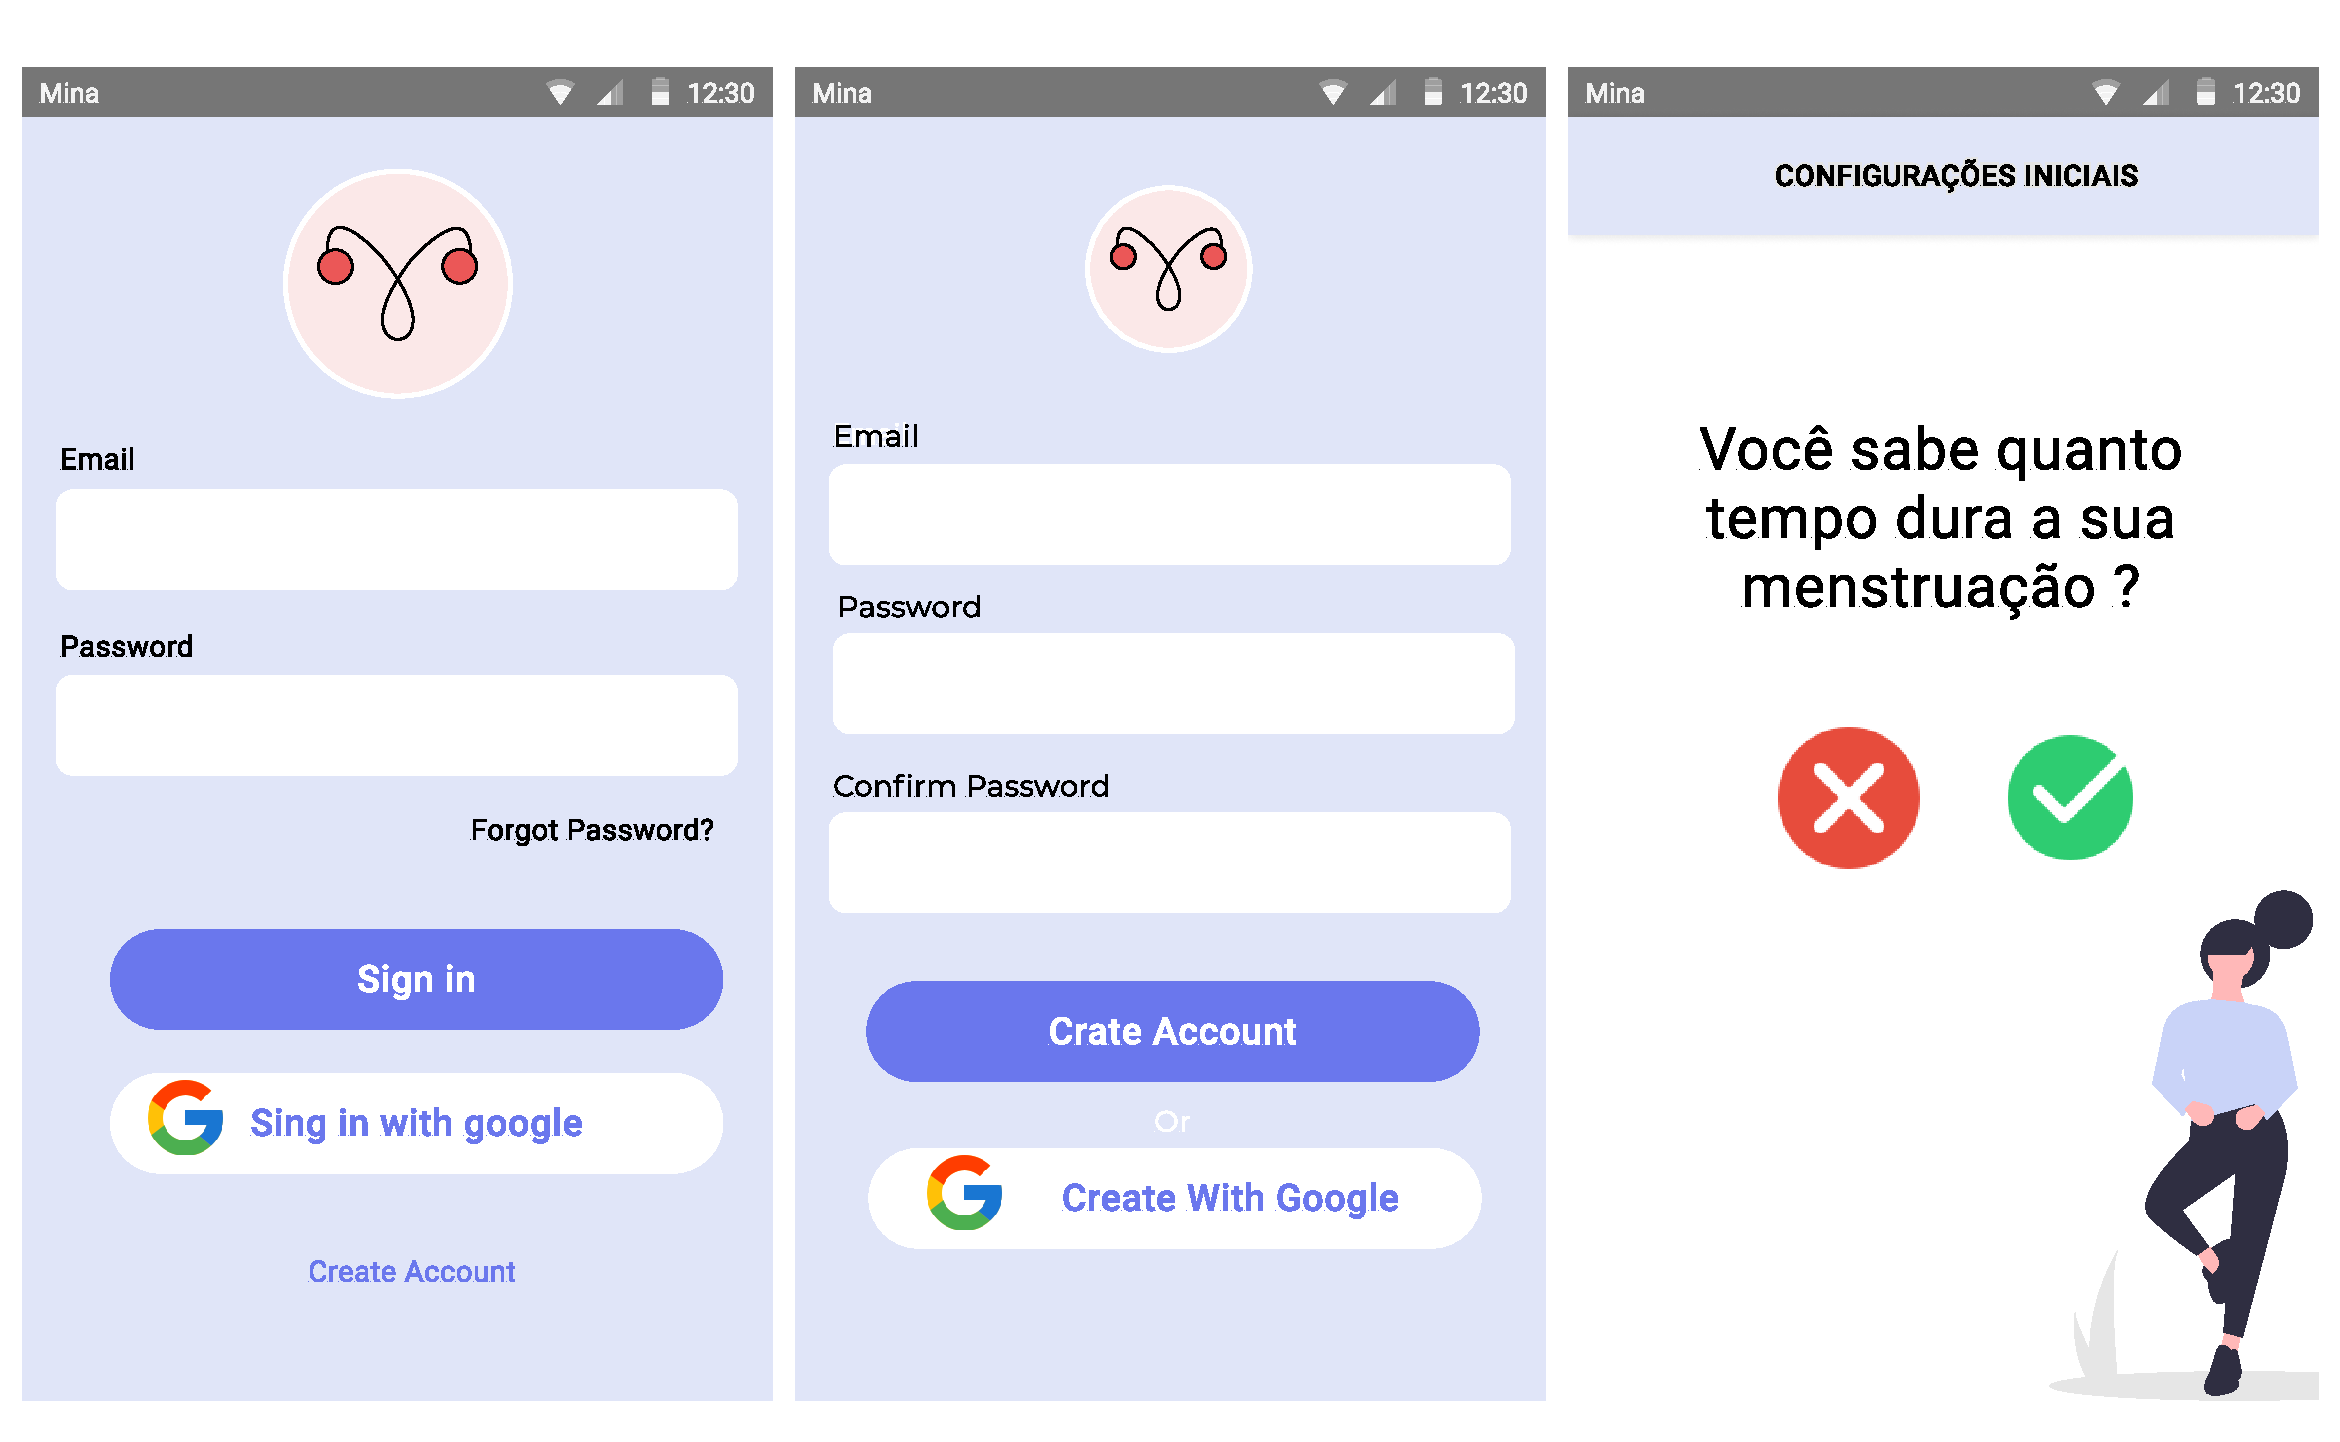
\includegraphics[keepaspectratio=true,scale=0.4]{figuras/prototipo1.pdf}
	\caption{Protótipo - Entrar, Criar Conta e Questionário}
        \label{fig09}
\end{figure}


\begin{figure}[h]
	\centering
	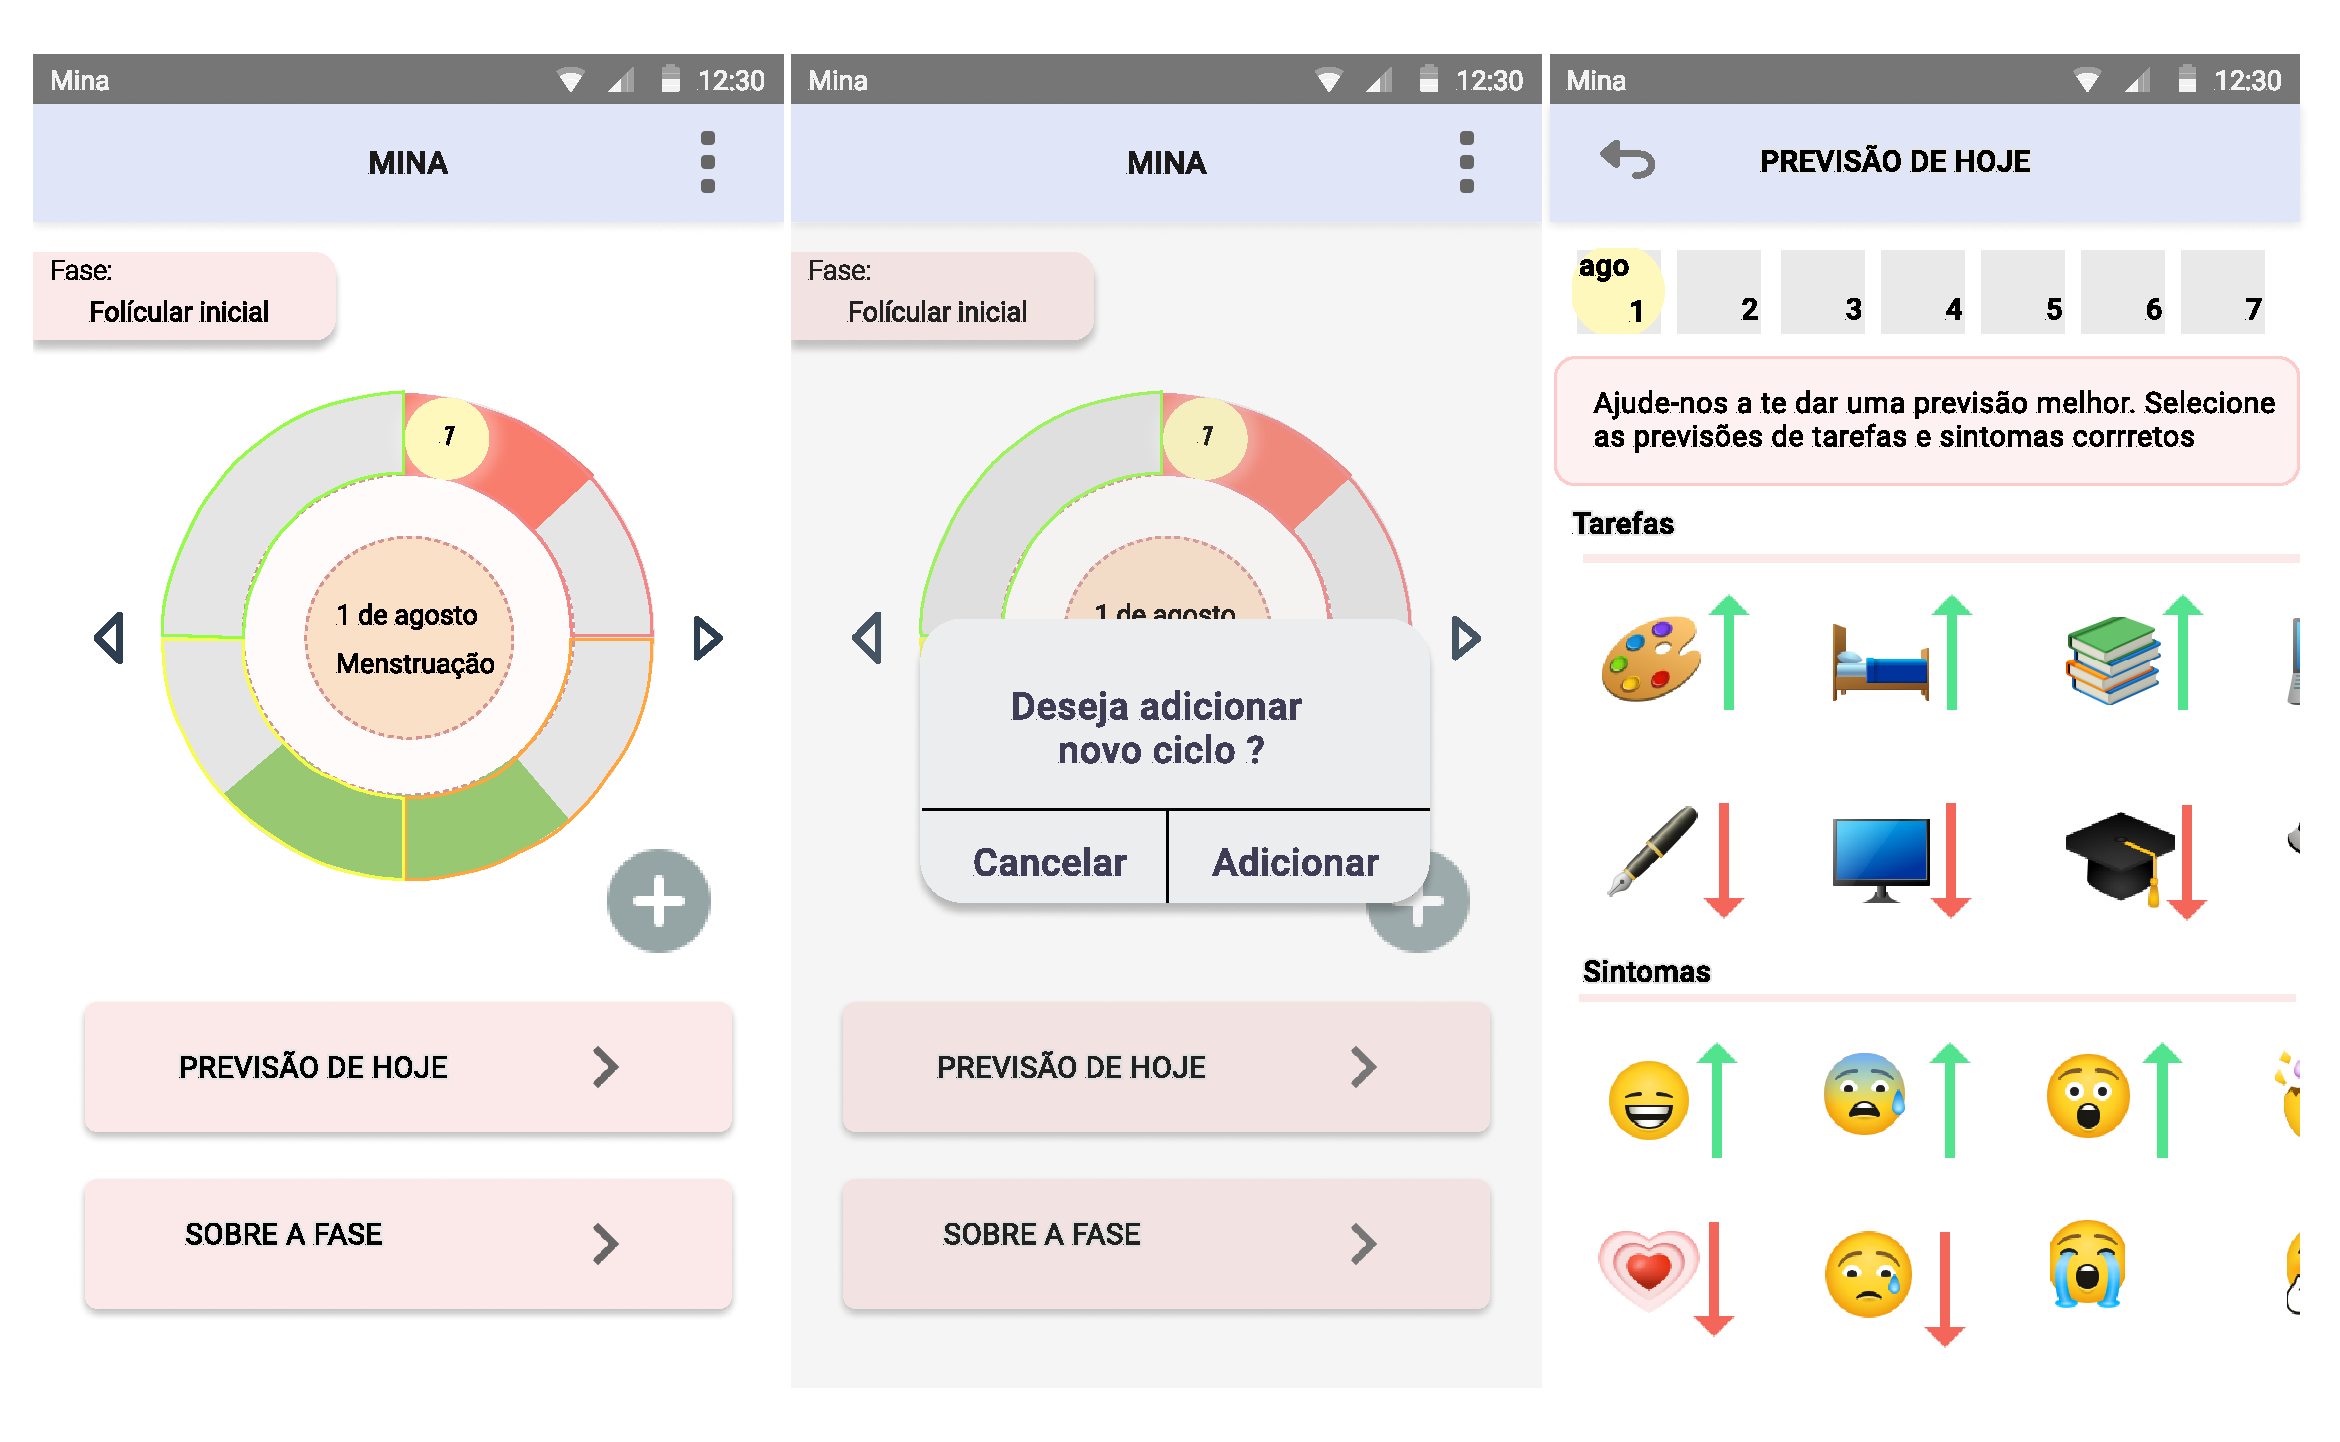
\includegraphics[keepaspectratio=true,scale=0.4]{figuras/prototipo2.pdf}
	\caption{Protótipo - Página Principal, Adicionar Ciclo e Previsão do dia}
        \label{fig10}
\end{figure}



\begin{figure}[h]
	\centering
	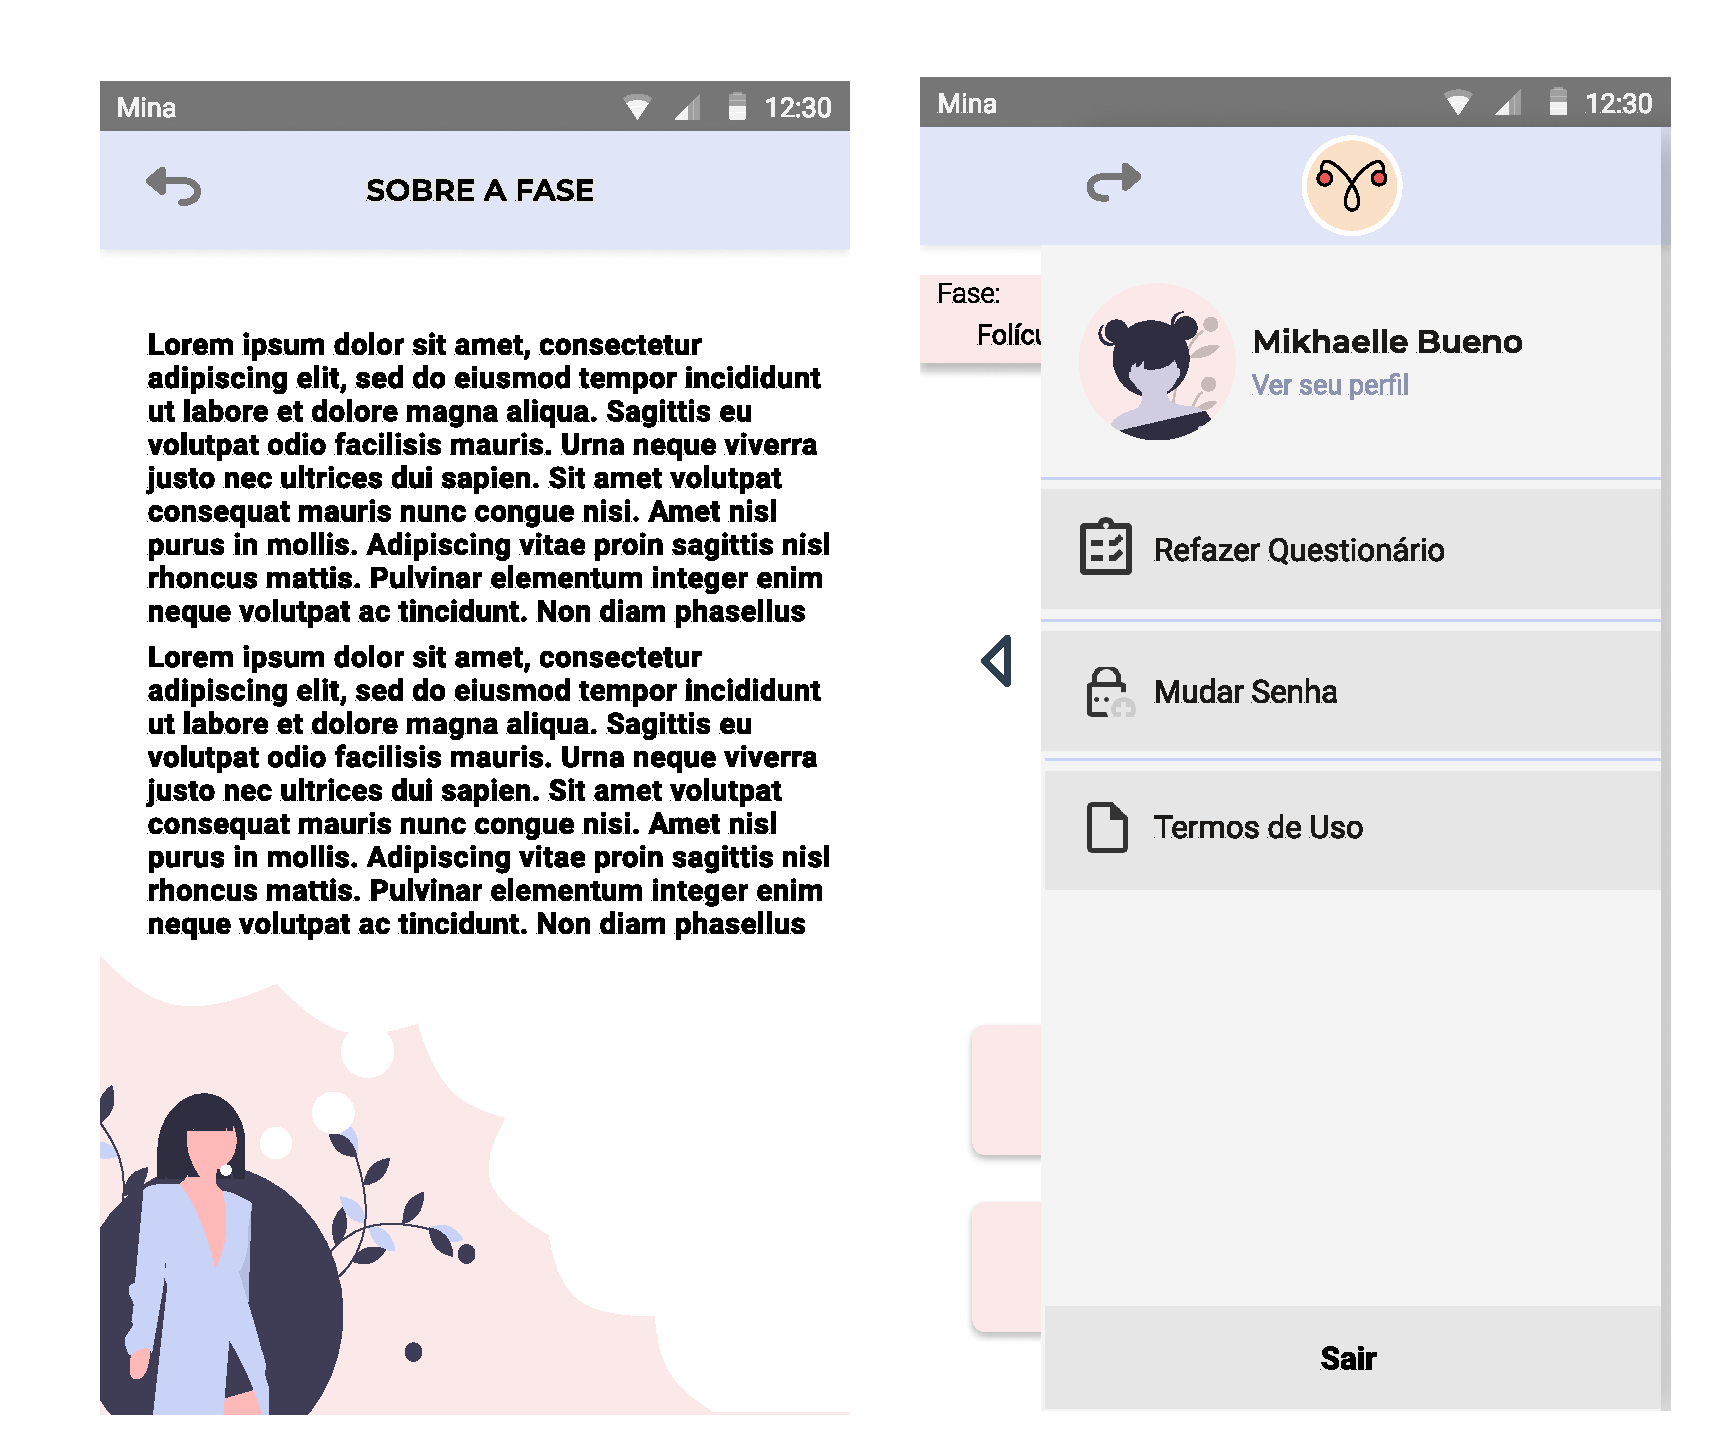
\includegraphics[keepaspectratio=true,scale=0.4]{figuras/prototipo3.pdf}
	\caption{Protótipo - Sobre a Fase e Perfil}
        \label{fig11}
\end{figure}


\subsubsection{Desenvolvimeno Inicial do Aplicativo}
O aplicativo está sendo desenvolvido com Flutter e Firebase e 
já teve 
ambas as tecnologias integradas. Inicialmente, para essa prova 
de conceito, 
foi desenvolvido um esboço inicial da tela principal (vide 
Figura \ref{fig12})

\begin{figure}[h]
	\centering
	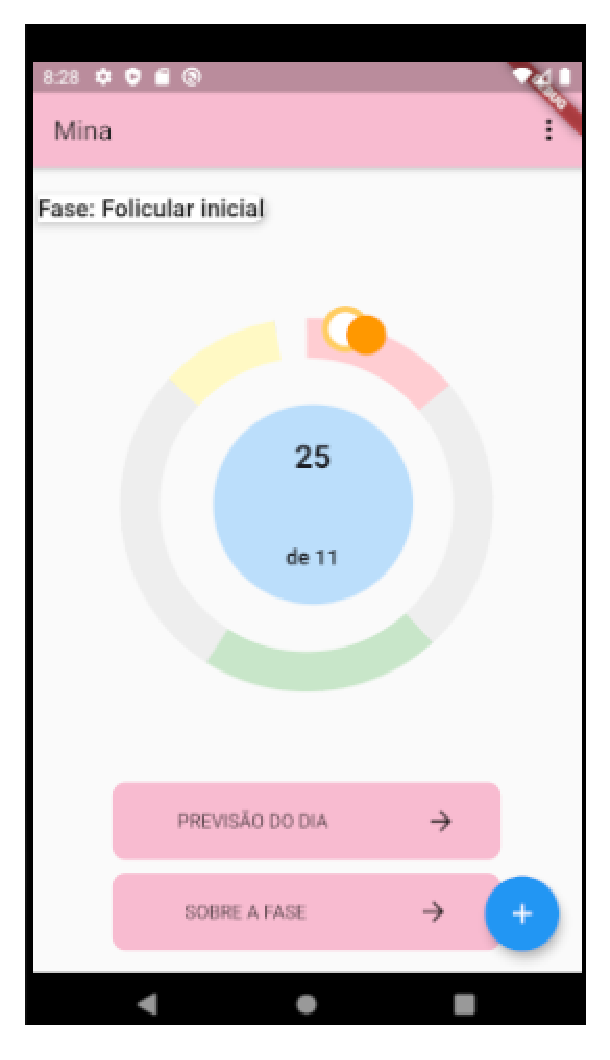
\includegraphics[keepaspectratio=true,scale=0.6]{figuras/apk1.pdf}
	\caption{Tela Principal do Aplicativo}
        \label{fig12}
\end{figure}

\section{Considerações Finais do Capítulo}

Neste capítulo, foi descrito o processo da tomada de decisão 
da ideia para 
esse trabalho na seção de considerações iniciais. Na seção 
de coleta de dados, 
foi descrito o processo de definição do aplicativo como 
plataforma e o primeiro questionário 
para coleta de dados. Na seção de análise de dados, foram 
listados alguns perfis identificados 
com a análise de dados do questionário e classificadas as 
tarefas que demandam mais ou menos energia 
para serem executadas de acordo com a fase do ciclo menstrual. 
Esse processo levou em consideração 
as respostas do questionário e a referência bibliográfica. 
A seção do aplicativo trouxe os requisitos elicitados e 
uma primeira versão de um \emph{produto backlog}. O aplicativo também conta 
com a prova de conceito, a qual focou na elaboração de um protótipo de alta fidelidade 
bem como o desenvolvimento 
inicial 
da aplicação, já dispondo do ambiente de desenvolvimento configurado e da tela 
principal. Por fim, cabe colocar que o aplicativo será chamado Mina. Esse estudo servirá como base para a execução 
do TCC2.